\chapter{Current status}
With the current work progress, the platform can be potentially deployed for tutoring a learner with the compiler development tools and basic concepts of compiler development including lexical analysis and syntax analysis. The exact details of the stages are as follows: 
\section{LEX Documentation}
A LEX document for the lexical analysis phase has been designed, compiled and reviewed. 
\section{YACC Documentation}
A YACC document for the syntax analysis phase has been designed, compiled and reviewed.
\section{LEX-YACC Documentation}
A LEX-YACC document for using YACC effectively with LEX has been designed, compiled and reviewed.
\section{Attributes Documentation}
A document on using the attribute stack of YACC has been designed, compiled and reviewed.  
\section{Extensions to SIL}
SIL is a strictly typed language with support for integer and boolean types alone. Currently does not provide support for user-defined types. In this section, we have proposed a language construct called "newtype" which can be used to create user defined data types in SIL.

"newtype" is a new language construct which can be used in the below shown syntax:
\begin{verbatim}
newtype
	typename
	{
		datatype variable_name;
		datatype variable_name;
	}
endtype			
\end{verbatim}
Each new user defined type can have upto a maximum of 8 variables which are either of a built-in data type or or a already defined user-defined data type. The syntax rules and the evaluation rules of the language construct have been provided in the "Appendix". 

The new types will be stored in a data structure similar to the symbol table, called the Type table. A sample type table looks like this:
\linebreak
\begin{center}
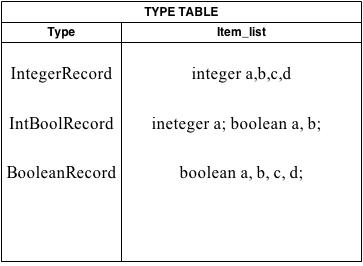
\includegraphics[width=0.4\textwidth]{./type_table.jpg}\\[1in]
\end{center}


\section{Online Platform}
The development of the mainframe of the website has been completed. All the completed documents are available online. Other components of the website are currently under construction. 

\chapter{APPENDIX}
\section{Syntax rules for "newtype"}
The syntax for the "newtype" construct has been provided below. We have used the YACC rules specification to express the syntax.

\begin{verbatim}
%token NEWTYPE VAR INTEGER BOLEAN

%%
typedef			: NEWTYPE typename '{' declaration_list '}' ENDTYPE
				;

declaration_list: declaration_list declaration
				| declaration
				;

declaration		: typename list_var ';'
				;

list_var		: list_var ',' VAR	
				| VAR				
				;

typename		: INTEGER
				|	BOOLEAN
				| VAR   
				;
				
%%
\end{verbatim}

\section{Evaluation rules for "newtype"}
The evaluation rules for the "newtype" construct has been provided below. We have used the YACC rules specification to express the semantics.

\begin{verbatim}
%{

/* Every item-list in the type table*/
struct table_entry
{
	char* id_name;							/* name of variable */
	char* type;								/* data type of variable */
	int binding;							/* address of the variable in memory*/	
	struct table_entry *next;				/* pointer to next entry */
};

/* Every type entry in the type table */
struct type_table
{
	char* type;
	struct table_entry *item_list;
};

/* Head pointer of the type table*/
struct type_table *HEAD;

/*Function to add an item list to the type table */
void add_type (char* type, struct table_entry *item_list);

/*Function to add an item entity to the end of an item list */
struct table_entry *append (struct table_entry *item_list, struct table_entry *item_entity);

/* Fuction to make an item which can be added to the item list */
struct table_entry *list_entity (char *type, char *id_name);

/* Function which returns the number of items in an item list*/
int list_len (struct table_entry *item_list);

/* Function to flag an error */
void yyerror(char *s);

%}

%union{
	char *type;
	struct table_entry *tentry;			
}

%token NEWTYPE 
%token <type> VAR INTEGER BOLEAN 

%type <tentry> id list_var declaration declaration_list 
%type <type> typename
%%

typedef: NEWTYPE typename '{' declaration_list '}' ENDTYPE			
																										{ 	if(list_len($4)<=8)
																													if(!existing_type(typename))
																														add_type(typename, $4);
																													else
																														yyerror("type already exists");
																												else
																														yyerror("type contains too many items");		
																										} 
			;

declaration_list: declaration_list declaration    	{ $$ = append($1,$2); }
				| declaration						{ $$ = $1; }				
	;

declaration: typename { $<type>$=$1;} list_var ';'	{ $$ = $3; }
			;

list_var: list_var ',' {$<type>$=$<type>0;} id			{ $$ = append($1,$4); }
		| {$<type>$=$<type>0;} id						{ $$ = $1; }		
		;

id: VAR									{	$$ = list_entity($<type>0,$1); }
	;

typename: 	INTEGER						{ $$ = $1; }
		| BOOLEAN						{ $$ = $1; }
		| VAR  							{ $$ = $1; } 
				;

%%
/* Auxiliary function definitions */
\end{verbatim}